\documentclass[11pt]{article}
\usepackage{graphicx}
\begin{document}

\tableofcontents
\title{Classical Cryptography Algorithms}
\author{Rohan Mundhey}
\date{\today}
\maketitle



\section{\textbf{CAESAR CIPHER}}

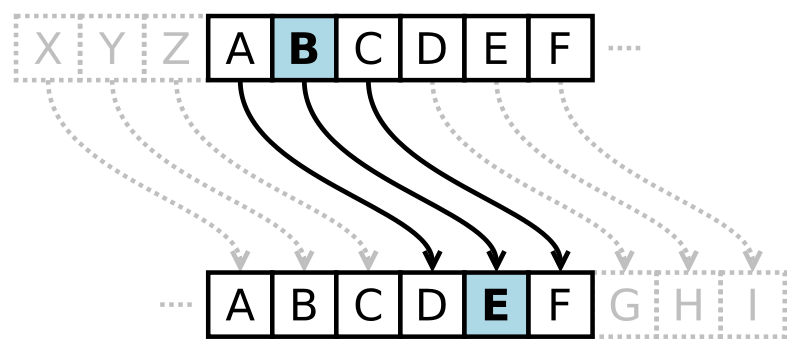
\includegraphics[width=5in,height=2in]{caesar_cipher.png}

The Caesar cipher, also known as a shift cipher, is one of the simplest forms of encryption. It is a substitution cipher where each letter in the original message (called the plaintext) is replaced with a letter corresponding to a certain number of letters up or down in the alphabet.
In this way, a message that initially was quite readable, ends up in a form that can not be understood at a simple glance.
For example, here's the Caesar Cipher encryption of a message, using a right shift of 3.
\\
\\
Plaintext:  
THE QUICK BROWN FOX JUMPS OVER THE LAZY DOG
Ciphertext: 
QEB NRFZH YOLTK CLU GRJMP LSBO QEB IXWV ALD
\\
\\
As unreadable as the resulting ciphertext may appear, the Caesar Cipher is one of the weakest forms of encryption one can employ.
\\
The key space is very small. Using a brute force method, one could easily try all (25) possible combinations in order to decrypt the message without initially knowing the key.
\\
The structure of the original plaintext remains intact. This makes the encryption method vulnerable to frequency analysis - by looking at how often certain characters or sequences of characters appear, one can discover patterns and potentially discover the key without having to perform a full brute force search.
\\
The Caesar Cipher can be expressed in a more mathematical form as follows:
$$E_n(x)=(x+n)mod26$$
\\
In plain terms, this means that the encryption of a letter x is equal to a shift of x + n, where n is the number of letters shifted. The result of the process is then taken under modulo division, essentially meaning that if a letter is shifted past the end of the alphabet, it wraps around to the beginning.
\\
\\
Decryption of the encrypted text (ciphertext) would be defined similarly, with instead a subtraction of the shift amount.
\\
$$D_n(x)=(x-n)mod26$$
\\
First used by Julius Caesar, the Caesar Cipher is one of the more well known older historical encryption methods. While you certainly wouldn't want to use it in today's modern world, a long time ago it might have done the trick.
\\
\\
\textbf{Algorithm}
\\
1.Begin\\
2.Declaration of Variables\\
3.message to be read\\
4.letters of message are to be shifted by 3 value\\
5.print pltxt //pltxt is now the required ciphertext\\
6.stop

\section{\textbf{ROT 13 CIPHER}}

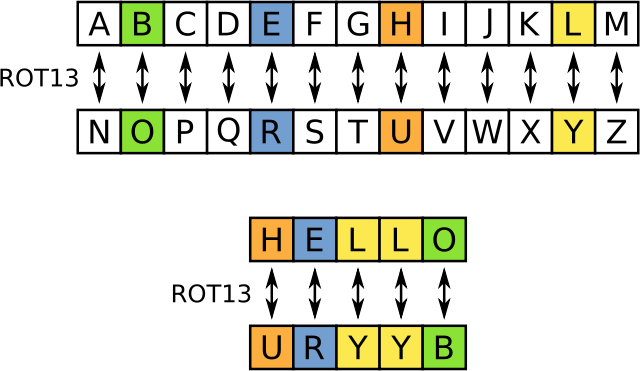
\includegraphics[width=5in,height=2in]{ROT13.png}

ROT13 ("rotate by 13 places", sometimes hyphenated ROT-13) is a simple letter substitution cipher that replaces a letter with the letter 13 letters after it in the alphabet. ROT13 is a special case of the Caesar cipher, developed in ancient Rome.
\\
\\
Because there are 26 letters in the basic Latin alphabet, ROT13 is its own inverse; that is, to undo ROT13, the same algorithm is applied, so the same action can be used for encoding and decoding.
\\
\\
Applying ROT13 to a piece of text merely requires examining its alphabetic characters and replacing each one by the letter 13 places further along in the alphabet, wrapping back to the beginning if necessary.
\\
\\
\textbf{Algorithm}
\\
\\
1.Begin\\
2.Declaration of Variables\\
3.message to be read\\
4.letters of message are to be shifted by 13 value\\
5.print pltxt //pltxt is now the required ciphertext\\
6.stop







\section{\textbf{VIGENERE CIPHER}}

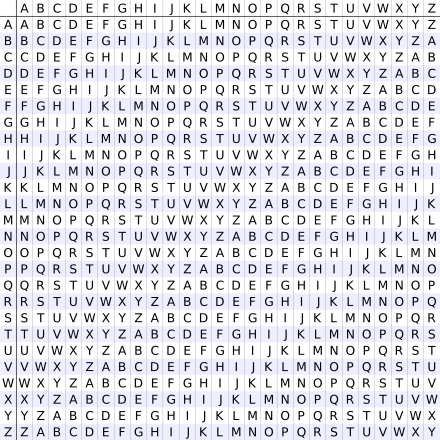
\includegraphics[width=5in,height=4in]{abc.jpg}

The Vigenère Cipher was developed by mathematician Blaise de Vigenère in the 16th century. The Vigenère Cipher was adapted as a twist on the standard Caesar cipher to reduce the effectiveness of performing frequency analysis on the ciphertext. The cipher accomplishes this using uses a text string (for example, a word) as a key, which is then used for doing a number of alphabet shifts on the plaintext. Similar to the Caesar Cipher, but instead of performing a single alphabet shift across the entire plaintext, the Vigenère cipher uses a key to determine several different shift amounts across the entirety of the message.
\\
\\
Should the key be shorter than the plaintext, it is repeated until the length matches. In this way, each letter in the plaintext is shifted by the alphabet number of the corresponding letter in the key.
\\
\\
Plaintext:  ATTACKATDAWN\\
Key:        LEMONLEMONLE\\
Ciphertext: LXFOPVEFRNHR
\\
\\
Expressed mathematically, the encryption of the message at letter i, is equal to the alphabetic value of i in the plaintext plus the alphabetic value of the corresponding i in the key.
$$E_k(M_i)=(M_i+K_i)mod26$$
\\
\\
Decryption is the same process reversed, subtracting the key instead of adding to arrive back at the original, plaintext value.
\\
$$D_k(C_i)=(C_i-K_i)mod26$$
\\
The Vigenère cipher was an improvement upon previous historical encryption techniques, but is still vulnerable brute force attacks and frequency analysis, though to lesser degree than the Caesar Cipher.
\\
\\
\textbf{Algorithm}
\\
1.Begin\\
2.declare variables\\
3.read plaintext and key\\
4.shift each plain text character by key character\\
5.print the cipher text\\
6.stop\\
\\
\\


\section{\textbf{ATBASH CIPHER}}

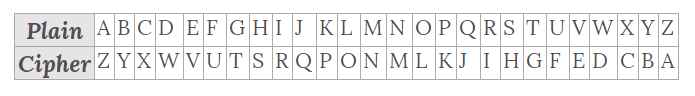
\includegraphics[width=5in,height=0.9in]{atbash.png}

Atbash is a monoalphabetic substitution cipher originally used to encode the Hebrew alphabet. It can be modified for use with any known writing system with a standard collating order.
\\
\\
The Atbash cipher is a particular type of monoalphabetic cipher formed by taking the alphabet (or abjad, syllabary, etc.) and mapping it to its reverse, so that the first letter becomes the last letter, the second letter becomes the second to last letter, and so on.
\\
\\
A few English words also 'Atbash' into other English words: "irk"="rip", "low"="old", "hob"="sly", "hold"="slow", "holy"="slob", "horn"="slim", "glow"="told", "grog"="tilt" and "zoo"="all". Some other English words 'Atbash' into their own reverses, e.g., "wizard" = "draziw."
\\
\\
\textbf{Algorithm}
\\
1.Begin\\
2.declare variables\\
3.read plaintext\\
4.replace each plaintext character according to table\\
5.print the cipher text\\
6.stop\\
\\
\\


\section{\textbf{ONE TIME PAD}}

Towards the end of the 19th century, it was becoming fairly obvious that simple substitution ciphers that were vulnerable to frequency analysis were no longer secure. How could they transmit a message without it’s contents being vulnerable to inspection, while still being able to be decrypted once they reached their destination? The answer is randomness.
\\
\\
Let’s consider a modified version of the Vigenère cipher as an example. Instead of performing alphabet shifts on each character in the plaintext via a key, we shift every character in the plaintext a random amount – with each of these random shift amounts becoming the resulting key. This results in a completely random key the exact same length as the original plaintext. This means that across the entire message, there can be no structure deduced from the frequency of characters, as the key itself was entirely randomly created. This type of encryption is called the one time pad, and the benefits don’t stop there.
\\
\\
With each character now having it’s own individual and random shift amount, the keyspace grows exponentially for each character in the message. Let’s say we were to encrypt the name “Alice” with a one time pad. That’s 5 letters – so to brute force it you would have to try a whole lot of possibilities:
\\
\\
$$(26x26x26x26x26) or 26^5 = 1188176$$
\\
\\
However, this would simply brute force the search space. You still wouldn't know which of the millions of attempts you tried were correct, because (due to the randomness of the one time pad) it's possible that attempting to decrypt the message with an incorrect key, could potentially give a coherent but incorrect result. Because of this, while being a relatively simple encryption technique, the one time pad is considered unbreakable if used properly.
\\
\\
There are however, downsides to the one time pad that should always be considered. The key size is always identical to the size of the message – which for long messages eventually becomes a lot of data to manage and a long encryption/decryption process. It also relies on a source of randomness, which can be exploited if not generated in a truly random fashion.
\\
\\
\\
\textbf{Algorithm}
\\
1.Begin\\
2.declare variables\\
3.read plaintext\\
4.Generate random text of size same as plain text\\
4.replace each plaintext character by random text\\
5.print the cipher text\\
6.stop\\
\\
\\

\section{\textbf{Cryptanalysis of ONE TIME PAD}}
Cryptanalysis is a process we use to analyse the cipher text and decode it to know the plain text.\\
In case of OTP (One time Pad) suppose our plain text is of size n ,then we generate a random key of same size n
,using this random key we shift each character of plain text to obtain the cipher text.\\
Now if we know only the cipher text then we can calculate it's size and generate all possible keys of that size ,using these keys we can apply the decrption algorithm to arrive at the plain text.
\\
\\
Example\\ 
Cipher text:ANGMP\\
length of Cipher text is 5\\
\\
No of keys to check : 26 * 26 * 26 * 26 * 26 = 11881376 

\end{document}